\chapter{Introduction}
\label{ch:introduction}

Software Engineering is the application of a systematic, disciplined, quantifiable approach to the development, operation and maintenance of software \citep{Acm:2015}. The challenges of educating new software engineers is more than just programming, they include attention to details, such as quality, schedule, and economic goals \citep{Acm:2015}. For instance, an important challenge in Software Engineering education arises from the dual nature of the Software Engineering discipline: it has roots in computer science and has emerged as an engineering discipline, and it affects both theory and practice \citep{Acm:2015}. This characteristic has a direct impact on the amount of material instructors must cover in Software Engineering classrooms. In addition, software professionals are required not only to understand technical challenges but also to be up-to-date with nontechnical issues, including management, communication, and teamwork.

In higher education, besides learning theory and acquiring technical skills, students need to develop the ability to apply, evolve, and practice those skills throughout their lifetime \citep{Gary:2015}. Additionally, soft skills, such as leadership, teamwork, decision-making, negotiation, and self-reflection, are important abilities for software engineering practice, since software development also involves several human and social aspects \citep{Marques:2014}. Nevertheless, the development of these crosscutting capabilities is usually less supported in computer science programs \citep{Marques:2014}.

There is no consensus on how to teach Software Engineering, since each institution adopts their own methods based on the experience of its professors \citep{Marques:2014}. Traditional approaches (expository lectures, exams, and complimentary assignments) are still largely used by lecturers \citep{Marques:2014, Bessa:2012,Prikladnicki:2009}. A possible cause is the difficulty in changing the instructional process used by the lecturers, and that it is a common pattern in computer science and engineering courses \citep{Marques:2014}. However, it may lead to demotivating students \citep{Prikladnicki:2009,Bessa:2012, Barnes:2008}. In addition, teacher-centered educational methods may not support the practical development of competences \citep{Barnes:2008} and may have limited learning efficiency \citep{Prikladnicki:2009}. Therefore, student-centered approaches may be more suited for allowing the development of competences as they learn-by-doing, with a higher motivation from the learner, a more active role in learning process, and better learning in the application level \citep{Prikladnicki:2009}.

ACM/IEEE Curricula Guidelines for software engineering programs – SE 2014 \citep{Acm:2015} – recommend including team-based projects into the software engineering and computer science curriculum. The necessity of providing real world experience of software development to students is a recurring theme on SE 2014, and several of its guidelines address this matter \citep{Acm:2015}. Curriculum Guideline 5 suggests that “students also need practical material to be taught early so they can gain maturity by participating in real-world development experiences (…)” \citep{Acm:2015}. Curriculum Guideline 10 discusses the multiple dimensions of the problem-solving aspect of software engineering, and suggests that “problem solving is better learning through practice and taught by example” \citep{Acm:2015}. Curriculum Guideline 17 suggests the need of using interesting, concrete and convincing examples to motivate students. Finally, Curriculum Guideline 14 objectively declares “the curriculum should have a significant real-world basis” \citep{Acm:2015}.

Several learning approaches have been proposed and applied to introduce practical aspects in SE education \citep{Marques:2014}, including: game learning, case studies, simulation, inverted classrooms, maintenance projects, service learning, and open source development. The applied nature of software engineering  has also motivated the adoption of game-related approaches for software engineering education \citep{Souza:2018}.

\section{Problem and Motivation}
\label{sec:problem}

A recurring challenge in Software Engineering (SE) education is engaging students to experience the professional practices of software engineering in such a way that they can understand which practices and techniques are useful in various different situations \citep{Acm:2015}. However, it is difficult to achieve the appropriate balance between theory and practice. This leads to a gap between the skills of recent graduates and the expectations of the software industry the software industry with the level of preparation of the recently graduated professionals \citep{Radermacher:2014}, specially regarding the lack of necessary competences to start performing their activities efficiently \citep{vonWangenheim:2009, Moreno:2012, Meira:2015}. Therefore, there is a gap between learn by studying (in academia) and learn by doing (at work) \citep{Moreno:2012}.

Software engineering courses in Computer Science or Information Systems departments usually provide limited opportunities for understanding the details related practices such as project management, quality assurance, and clients requirements understanding [PEIXOTO 12]. Software processes, for instance, play a key role in SE Education, both as a focal and as a crosscutting topic to reinforce students’ understanding of software engineering practice \citep{Acm:2015}. However, students practice of software process in academia is limited to the practical assignments they are exposed during academic life (such as project-based activities, capstone projects, and practical exercises). In addition, the nature of these assignments and projects proposed in the classroom is limited in scope and time.  Therefore, incorporating real-world elements into the curriculum is a crucial challenge to enable effective learning of software engineering skills and concepts \citep{Acm:2015}.

The curriculum guidelines of the ACM/IEEE \citep{Acm:2015} emphasize that the professional competences emerge through the theoretical study of knowledge units and the practical application of their concepts. As a consequence, it is necessary to move beyond the expository classroom format, since it does not favor effective student learning \citep{Acm:2015}. These guidelines also suggest the importance of introducing real world problems, related to SE, in the learning process, and the inclusion of knowledge units that allow the development of the competences expected for professionals in the area.

In the instructor perspective, however, developing professional competencies in students using practical assignments is challenging, because it requires that: (i) instructors understand and plan the expected outcomes in terms of skills the students are supposed to develop; (ii) instructors specify processes, activities, policies or procedures that allows and induce students to develop specific skills; (iii) students are properly trained or mentored for executing the specified process, activities or procedures in order to develop the expected skills; (iv) instructors evaluate the outputs of students activities for assessing the development of skills. Additionally, it is important that students are well motivated to perform these activities.

One strategy that has been largely used to overcome these challenges is the introduction of software projects in software engineering education (eg.: capstone and project-based courses) \citep{delgado:2017, marques:2017}. In this context, project-based learning is one of the main successful student-centered educational approach broadly used in computing science, information systems and engineering courses \citep{delgado:2017, marques:2017, Macias:2012, Jazayeri:2015, Shuto:2016, Warin:2016, Yamada:2014}. However, there is a shortage of comprehensive methodological frameworks and tools \citep{Warin:2016, Macias:2012}. As a consequence, it may aggravate other problems related to PBL adoption, such as: the effort required to run PBL courses \citep{Harms:2016, Hanakawa:2015, Nguyen:2013, marques:2017, Rupakheti:2017, Daun:2016, Gary:2015, Makio:2017}; scalability \citep{Harms:2016, Gary:2015}; and the difficulty to track students progress through the project \citep{Fukuyasu:2013, Harms:2016}.

Gamification, in the other hand, has been used in software engineering educations as a strategy to engage and motivate students in performing specific behaviours, such as the more frequent use of specific tools, acquiring the habit of applying specific techniques, or being more participative in the classroom. Gamification has also been used as a strategy to induce learners to use specific software engineering abilities or practices, by promoting competition or systematically rewarding learners as they perform expected actions or show expected behaviors. Therefore, it is a relevant strategy to support students in developing an appreciation of the importance of continued learning and in acquiring habits for professional software development \citep{Souza:2018}. Similar to PBL, a problem related to Gamification is the difficulty of adapt it to each context, as there are few studies providing general guidelines to use this technique for software engineering education.

Therefore, the motivation for using specific methods and approaches in learning process is influenced by  several  criteria,  for  instance, the flexibility and ease of using the approaches, their  suitability  for  being  used  by  most  instructors,  and  the  effort,   restrictions  and  skills  involved  in  the  use  of  these  approaches \citep{Marques:2014}. For instance, in a survey with 89 SE professors about the adoption of games and game elements in SE education [APÊNDIX A], the most recurring cause of not using these approaches were related to: the lack of knowledge (21.3\%); not knowing appropriate games for SE education (15.7\%); lack of time (13.5\%); not believing in the method (6.7\%); lack of interest in the method (5.6\%); lack of materials to support the adoption of this method (4.5\%); lack of resources (2.2\%). Even considering that the use of games in software engineering education is not new \citep{Souza:2018}, the lack of approachable models for introducing alternative learning methods is still a barrier. Thus, providing educators with appropriate resources to support the adoption of alternative learning methods may contribute to addressing the problems previously mentioned.

As a consequence, the motivation of this thesis project lies on: (i) the necessity of introducing practice in SE education and the related challenges; (ii) the gap between what and how SE is taught in university and the competences needed from professionals entering the industry; (iii) the necessity of moving beyond expository lectures; and (iv) the need of approachable materials and resources to support educators in the introduction of alternative student-centered educational methods. 

\section{Goals}
\label{sec:goals}

The goal of the thesis is to propose a conceptual framework to support the gamification of project-based software engineering education. This framework is intended to provide guidelines on how to setup educational software development projects, using Gamification to guide and motivate students on performing specific process activities. To achieve this goal, the following specifics goals are defined:

\begin{itemize}
    \item Study the literature related to Software Engineering education;
    \item Investigate the use of PBL to support Software Engineering Education;
    \item Investigate the use of Gamification to support Software Engineering Education;
    \item Define a Framework for the Gamification of project-based software engineering education;
    \item Evaluate the proposed framework.
\end{itemize}

The goal of this research is not defining a novel educational method for SE education, but to integrate existing approaches (PBL and Gamification) in an unified approach.

The scope of this thesis is limited to the investigation of PBL and Gamification in the context of SE education. Although we acknowledge the existence and relevance of other methods and techniques to support SE education,it is out of the scope of this thesis the comparison of the approach proposed in this thesis project to other approaches.

\section{Research Questions}
\label{sec:questions}

Based on the research goals of this Thesis, the following research questions are defined:

\begin{itemize}
    \item \textbf{RQ1} How can Gamification be used to support software engineering education?
    \item \textbf{RQ2} How can PBL be used to support software engineering education?
    \item \textbf{RQ3} What are the benefits of using Gamification and PBL in conjunction to support software engineering education?
\end{itemize}   

\section{Method}
\label{sec:method}

This thesis adopts the design science paradigm. The design-science paradigm seeks to extend the boundaries of human and organizational capabilities by creating new and innovative artifacts. In the design-science paradigm, knowledge and understanding of a problem domain and its solution are achieved in the building and application of the designed artifact [REFERÊNCIA]. 

The study design of this thesis is based in an multi-method approach that combines two or more quantitative or qualitative methods (HESSE-BIBER, 2010). In this thesis we adopt secondary literature studies, Action-Research, and other empirical approaches. In this approach, data triangulation is used to consolidate results from different methods, in order to answer the Research Questions, and collect data from different sources to reinforce the study validity (EASTERBROOK ET AL., 2007).
 
Figure \ref{fig:method} presents the study design adopted for this thesis project. The research starts with the definition of the research problems, goals and questions, obtained from an initial literature review on the theoretical foundation of software engineering education and its methods. This review supported the identification of principles, concepts and methods for software engineering education, and contributed for the theoretical background of this thesis (Chapter \ref{ch:background}).
 
For the next steps, the research forked in two parallel investigations: (i) the investigation on the use of Gamification in software engineering education, and (ii) the investigation on the use of PBL in software engineering education. The first (i), resulted in a systematic mapping study of the literature to understand the state-of-the-art literature on the use of game-related methods used in software engineering education, and situate the use of Gamification in comparison to other methods (Chapter \ref{ch:sms}). Then, an empirical study was conducted for the use initial experimentation on the use of Gamification in an introductory software engineering course (Chapter \ref{ch:gamificationExperiment}). For the second (ii), a survey of the literature was performed to identify the main challenges of the use of PBL in software engineering education (Chapter \ref{ch:background}), and an Action-Research study was performed to empirically evaluate the use of this learning method in an introductory software engineering course (Chapter \ref{ch:actionResearch}). It is important to note that these investigations (i and ii) are not sequential.
 
Based on the lessons learned from the previous steps, a framework is currently being designed to support the Gamification of project-based software engineering education. The initial outline of the framework is presented in Chapter \ref{ch:framework}. The evaluation of the framework, planned as a final step of this thesis is not discussed in detail in this thesis project, however, initial thoughts on the planning of this step are discussed in Chapter \ref{ch:framework}.

\begin{figure}[!h]%th
\centering
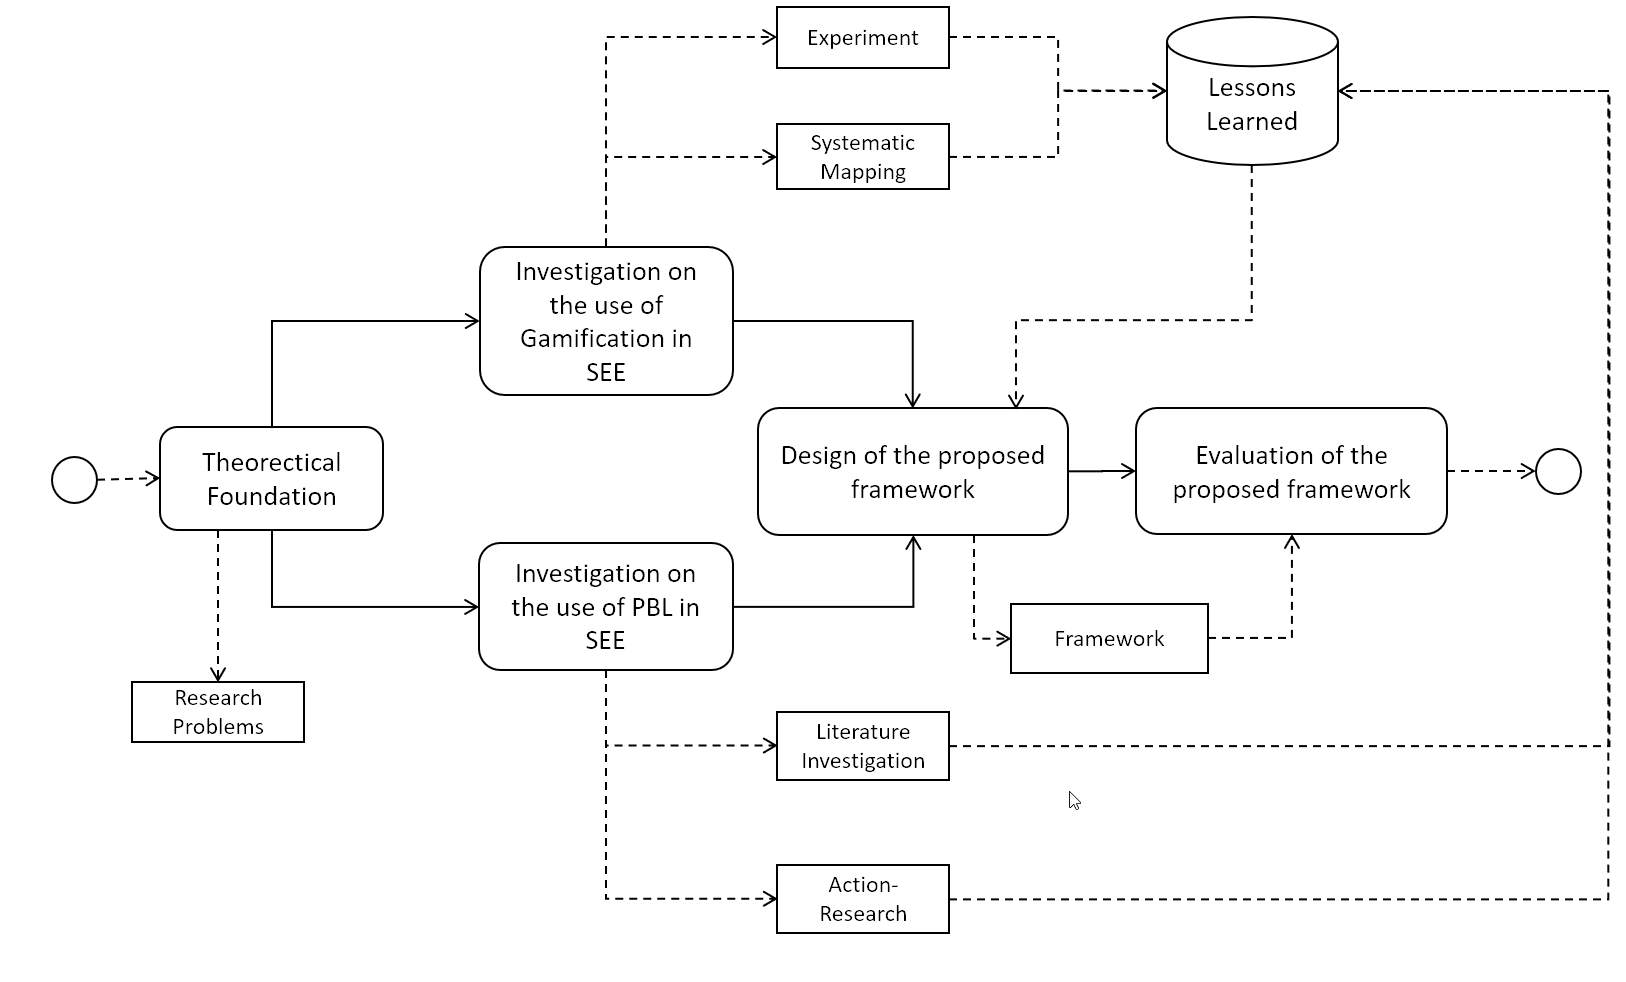
\includegraphics[width=1\textwidth]{img/method.png}
\caption{Study design}
\label{fig:method}
\end{figure} 

\section{Contribution and Relevance}
\label{sec:contribution}

The main expected contribution of this thesis is the documentation of a framework for the gamification of project-based software engineering education. This product is expected to provide educators with a reusable method and guidelines to support the introduction of educational software projects as practical assignments in SE related courses, grounded in lessons learned from theory and practice on the use of Gamification and PBL.

The relevance of this study relies on the growing demand for development of professional competences on undergraduate SE students, the recurring challenge of balancing theory and practice in SE education. As a byproduct of this thesis, this research contributes with additional options for the introduction of Gamification and PBL in SE education. Additionally, a recurrent problem stated in the literature on Gamification in SE education is the shortage of empirical evidences of the use of this technique. Therefore, the relevance and contribution of this thesis also resides in providing empirical data regarding the use of PBL and Gamification.

Until the date of production of this document, the following publications were byproducts of this thesis project:

\begin{itemize}
    \item Mauricio R. de A. Souza, Lucas Veado, Renata Teles Moreira, Eduardo Figueiredo, Heitor Costa. A Systematic Mapping Study on Game-related Methods for Software Engineering Education. Information and Software Technology (IST), ISSN 0950-5849, DOI:10.1016/j.infsof.2017.09.014. 2018.
    \item Maurício R. A. Souza, Lucas Veado, Renata Moreira, Heitor Costa, Eduardo Figueiredo. Games for Learning: Bridging Game-related Education Methods to Software Enginering Knowledge Areas. 39th International Conference on Software Engineering (ICSE), Software Engineering Education and Training (SEET) track. DOI: 10.1109/ICSE-SEET.2017.17. Buenos Aires, Argentina, 2017.
    \item Maurício R. A. Souza, Kattiana Constantino, Lucas Veado, Eduardo Figueiredo. Gamification in Software Engineering Education: An Empirical Study. 30th International Conference on Software Engineering Education and Training (CSEE\&T).  DOI: 10.1109/CSEET.2017.51. Savannah, GA, USA, 2017.
\end{itemize}

This project also resulted in the following presentation:

\begin{itemize}
    \item Maurício R A Souza, Renata Moreira, Eduardo Figueiredo. A Framework for the Gamification of Practical Assignments in SE Education (Poster). 30th International Conference on Software Engineering Education and Training (CSEE\&T). Savannah, GA, USA, 2017.
\end{itemize}

The following research papers have been submitted for conferences:

\begin{itemize}
    \item \textbf{Games and Gamification in Software Engineering Education: A Survey with Educators} - The results of survey with 83 software engineering professors from Brazilian universities regarding the adoption of game-related approaches in software engineering education.
    \item \textbf{Giving the Game Away: A Detailed Study of Game Elements} - The identification of the main game elements used to support software engineering activities (both in academia and industry), and proposal of a conceptual framework for their adoption.
    
\end{itemize}

\section{Thesis Project Outline}
\label{sec:outline}

In addition to this introductory chapter, Chapter 2 provides the essential concepts related to the research. Chapters 2, 3 and 4 presents investigations on the use of specific learning methods in software engineering education. Chapter 5 delineates the initial documentation of the framework proposed in this thesis project. The details on each chapter is presented as follows:\\

\noindent
\textbf{Chapter~\ref{ch:background}} presents background information to support the comprehension of this thesis project. It includes the main concepts related to software engineering education, learning methods adopted in SE education to support practice, and game-related methods used in SE education. This chapter also discusses related work.\\

\noindent
\textbf{Chapter~\ref{ch:sms}} presents the protocol and results of a systematic mapping study performed to identify the state-of-the-art literature on game-related educational methods to support software engineering education.\\

\noindent
\textbf{Chapter~\ref{ch:gamificationExperiment}} describes an empirical study on the adoption of Gamification in an introductory software engineering education.\\

\noindent
\textbf{Chapter~\ref{ch:actionResearch}} presents an Action-Research study describing the adoption of PBL in an introductory software engineering course and reports the lessons learned from this study.\\

\noindent
\textbf{Chapter~\ref{ch:framework}} presents the initial outline of the proposed framework to support the gamification of project-based software engineering education.\\ 

\noindent
\textbf{Chapter~\ref{ch:conclusion}} presents the conclusion of this thesis project, summarizing the status of the project, next steps, and the main lessons and issues found until the moment of conclusion of this document.